\documentclass{sig-alternate-05-2015}
\begin{document}

\setcopyright{acmcopyright}
\title{Mitigating signal handler exploits in Linux
\titlenote{(Produces the permission block, and
copyright information). For use with
SIG-ALTERNATE.CLS. Supported by ACM.}}
\numberofauthors{2}
\author{
\alignauthor
Abhiram Balasubramanian\\
       \affaddr{University of Utah}\\
       \email{abhiram@cs.utah.edu}
% 2nd. author
\alignauthor
Scott Bauer\\
       \affaddr{University of Utah}\\
       \email{sbauer@eng.utah.edu}
}

\maketitle
\begin{abstract}
As exploitation mitigations advance attackers look for new methods to control the flow of a program after exploiting a vulnerability. Recent exploit mitigations such as StackGuard \cite{cowan1998stackguard}, Data Execution Prevention \(W^X\) \cite{WXORX} and Address Space Layout Randomization (ASLR) \cite{ASLR}, have forced exploit authors to use techniques that jump around the text segment of an ELF in memory to achieve code execution. The newest form of exploitation, Sigreturn Oriented Programming (SROP), uses signal frames, and the kernel to achieve code execution by tricking the kernel to change the instruction pointer to some arbitrary location in the code.\\
Signals are one of the commonly used kernel to user/user to user asynchronous notification mechanisms in UNIX. By registering a signal handler, a process can handle these asynchronous events outside its control flow. As signal frames are stored on the process stack, attackers can create exploits by setting up dummy signal frames on the stack and initiate returns from signals that the kernel never delivered. This method bypasses all current exploit mitigation techniques and  appears more convenient as kernel never keeps track of the signals it delivered.\\
We develop a mechanism on top of the 4.1 Linux kernel to systematically stop SROP exploitation.

\end{abstract}
\section{Introduction}
Over the past 25 years Operating System designers and compiler designers have been facing off against exploit developers. The OS and Compiler designers  come up with a novel technique to suppress some form of exploitation method, for example Stack cookies, ASLR, DEP, etc. The exploit developers however continuously find methods around these exploit mitigations and the cat-and-mouse game continues.  A paper titled “Framing Signals -- A return to portable Shellcode”,  presents a new novel exploitation technique based off the idea of Return Oriented Programming (ROP). In a ROP an attacker locates gadgets in the assembly and continuously returns to those locations to build working shellcode. In this new technique attackers leverage the way Unix-like operating systems deliver signals to applications to create portable and reliable shellcode. This technique works by crafting a signal frame on the stack and tricking the kernel into thinking it is a legitimate signal frame. Doing so causes the kernel to transition control of the program to the location specified in the dummy signal frame, allowing an attacker an easy mechanism for arbitrary code execution.\\
\indent
To mitigate this new style of exploitation we design, implement and use a SROP mitigation technique based off of the idea of cookies originally developed to stop stack based buffer overflows. We test our implementation against two different SROP exploits, both of which are stopped by the new mitigation technique.

\section {Background}
<TBD>
\subsection{Signal Handling in Linux}
<TBD>
\subsection{Signal Return Oriented Programming}
notes: 
I want to mention how srop give an attacker a super easy way to populate registers in a controlling manner. In ROP to get good execution you have to coax values into registers via rop gadgets, if there are no gadgets that will populate the register the way you want you're SOL. But with SROP you just setup the sigframe the way you want and everything is good to go.
<TBD>
\section {System Implementation}
We classify the system implementation in two sections - construction
of the exploit and the kernel implementation to mitigate the exploitation.

\subsection{A simple SROP exploit}
We implemented an exploit by carefully constructing a stack frame to give
control to a shellcode. The key idea in creating this exploit is to make
the instruction pointer (IP) point to the code that we want to execute. 
Unlike return oriented programming, SROP needs to know the location of 
code that executes a sigreturn system call. To accomplish this, we simply
created a gadget function that respects the system ABI to execute a system
call. Essentially, the gadget sets the system register RAX with the syscall
number (0x15 for sigreturn) and calls syscall instruction to execute sigreturn.
See Figure~\ref{fig:SFEC} for more details.

\subsubsection{Finding gadgets}
\par The ideal way of constructing an attack is to find an address of a
syscall instruction in the system address map. Although the vsyscall area provides 
an address of a syscall instruction, on 64 bit kernels the area is emulated. 
The kernel has a mechanism to check if the syscall number was the one which the 
vsycall area supports to execute, if not, the kernel throws a SIGSEV error 
saying an exploit has been attempted.  
\par So, in order to get the exploit working, we placed a gadget with a syscall 
instruction and have the code point to this gadget instead of the vsyscall area.
Although there are other methods to find the syscall address, such as finding a 
syscall address in libc shared library, this method is more elegant and simple to 
construct the attack.

\subsubsection{Preparing arbitrary code execution}
In order to execute the shellcode, we first need to ensure that sigreturn system
call executes successfuly so that it restores the shellcode context later on. We
place a fake ucontext frame on stack such that it executes a execve instruction to
load shell. For this purpose, it is important to set the code segment register to 
point to 0x33 so that it runs in 64 bit mode, RAX set to syscall number of execve
system call, RDI and RSI points to the arguments (shell in our case) respectively.
When the executable is loaded, it overwrites the return address with the sigreturn
system call address and loads the fake ucontext frame to launch the shell.

\begin{figure}
\centering
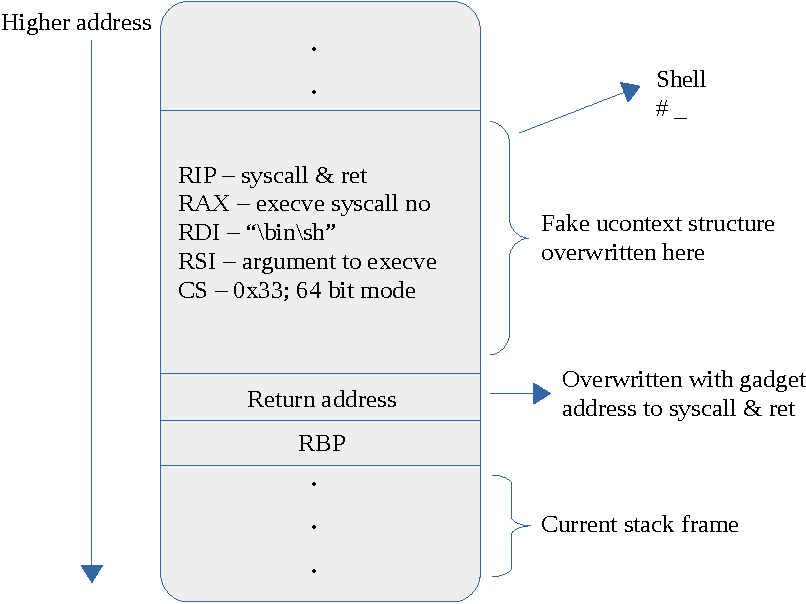
\includegraphics[height=2.5in, width=3in]{exploit}
\caption{Stack frame of exploit code}
\end{figure}

\subsection{Mitigating SROP}
To mitigate SROP exploits we need the kernel to remember or have the ability to derive whether or not the signal frame placed on the user stack is legitimate. A legitimate signal frame is a frame that was placed on the stack, by the kernel, during the delivery of a pending signal. If the kernel can determine the legitimacy of a signal frame it can then also detect signal frames that are apart of a SROP exploit, or buggy program. To give the kernel the ability to detect legitimate signal frames we place a cookie within the signal frame that will be audited during the \textit{sigreturn} system call. If there is no cookie in the frame, or the cookie in the frame doesn't match what the kernel expects, the process is gracefully terminated with a SIGSEV, more commonly known as a segmentation fault.
\subsubsection{Design Choices}
There are a series of design choices we have to make in order to build a defense mechanism that is fast, secure and most important to us, could be accepted by the upstream kernel developers. The decision to use a cookie within the signal frame comes from the stack buffer overflow mechanism in StackGuard. A cookie in the signal frame increases the length of the frame only by 8 bytes, a small price to pay for protections against an exploitation method. To verify the cookie during a \textit{sigreturn} system call we need to remember the cookies we've placed in the frame. One idea is to save every cookie in a list on the process' local storage struct. This method fails for multiple reasons. First being an attacker could send many signals to a process causing the list to get filled up with cookies, after a certian time the range of cookies in the list is very large, possibly allowing an attacker to guess a correct cookie in the list. The second reason this fails is in implementation details. In order to save the cookies in this mechanism the kernel would have to allocate memory for nodes in the linked list on the signal-fast path. More over, on the sigreturn path the kernel would have to walk a linked list, possibly quite large, searching for the cookie. Due to these implementation issues saving every cookie was quickly excluded. Another approach we designed, but quickly shot down, was to hash the entire signal frame and save the hash at the bottom of the signal frame. We quickly realized an attacker could hash their custom signal frame, place the hash at the bottom, thus tricking the kernel. We decided the following goals had to be met:\\
\begin{itemize}
  \item The kernel shouldn't have to remember every cookie it puts in a signal frame.
  \item The signal delivery code, and sigreturn code needs to remain fast.
  \item The only location the cookie should be saved is on the process' stack.
  \item The cookie should not be the same for every signal, even within the same process.
\end{itemize}
%To mitigate SROP the kernel needs to remember during signal delivery that a signal was sent to the userland process. That way during the \textit{sigreturn} systemcall the kernel can verify that it is actually handling the cleanup of a signal it sent. %
\subsubsection{Implementation}
To realize the goals outlined in the previous section we came up with the following implementation. Each process will generate a 64 bit secret during start up, the secret will be held in the process' control block. During delivery of a signal, the kernel will generate a cookie based on the 64 bit secret as well as the address, in user-land, of where the cookie will be stored. From there the kernel places the cookie at the address and continues with normal signal delivery. Upon execution of a \textit{sigreturn} system call, the kernel extracts the cookie from the frame, it then does the same calculation as above. If the calculated and extracted cookie differ then either the process broke the ABI by moving the signal frame, or there was an exploitation attempt. This implementation meets all the goals we outlined in the previous section. The kernel doesn't have to remember every cookie it places in a frame, it only has to remember a secret one . The signal delivery and signal return code remain fast, no memory allocations or costly list walks occur. The cookie changes for each signal due to the fact we use the memory address of where the cookie is to be stored in the actual cookie calculation.
\\
\indent
We implemented this protection mechanism on top of the 4.1 Linux tree, we selected 4.1 instead of mainline due to mainline not running correctly in our Xen virtual machine. We generate the cookie using the following code:
\\
\begin{verbatim}
/* Take address of sig cookie, xor with secret */
temp = &frame->sig_cookie ^ current->sigret_secret

/* hash the cookie */
sig_cookie = hash_64(temp);

/* place the hashed cookie on the users stack */
__put_user(temp, &frame->sig_cookie);

\end{verbatim}

To verify the cookie we do the following:

\begin{verbatim}

hashed_cookie;

__get_user(&hashed_cookie, &frame->sig_cookie);

/* do the same calculation as above */

...

if (hashed_cookie != calculated_cookie)
   send_SIGSEV();

....

\end{verbatim}

\section{Related Work}
For this work, \cite{bosman2014framing} is most relevant and a one 
stop reference. The paper provides detailed technical information 
on signal handling on UNIX based systems and introduces SROP as a 
generic exploitation technique. It also points to hints on abusing 
sigreturn system call, backdoor techniques based on SROP and ways to 
mitigate SROP attacks. 

\par In our current work, we have implemented a simple execve based 
exploit technique and a stack cookie based kernel level implementation
to address the exploitation as suggested in the paper. The paper authors
have also submitted a kernel patch targeting a different approach - counter
per process in the kernel space that keeps track of number of signal handlers
currently executing, the counter increases on signal delivery and decreases
on sigreturn path. Although this technique prevents SROP technique, it has
its own drawbacks in terms of counter roll-over and creates complications with
multi-threaded applications. We presume that these are some valid reasons why
the patch has not made it into the mainline kernel. In contrast, our approach 
is more elegant and leaves less to no room for the attacker to guess the cookie
value. Moreover, techniques suggested in the paper target older kernel versions, 
we have tested the exploit and the kernel fix on the latest kernel version (4.3).

\par As SROP is a type of an ROP attack, we find \cite{cowan1998stackguard}
related as this work implements a compiler feature which adds a cookie to the stack, 
as well as support to verify the cookie upon return of a function.  Buffer overflow 
attacks are probably the most famous form of attack gaining notoriety in the early 90's
The method works by modifying gcc such that it generates code that places a
32 bit identifier on the stack before the return address during a call instruction.
Also prior to a return gcc has the function call a verify method which validates 
that the 32 bit identifier is the same identifier that was placed there previously.
This research is very similar to the approach we have taken to prevent SROP.  
We utilize a stack cookie generated by the kernel to prevent an attacker from 
creating an arbitrary signal frame on the stack causing the kernel to jump arbitrarily 
through the code.

\par Another relevant reference is \cite{li2010defeating} as the work implements a 
compiler technique to prevent ret instructions from being generated in a kernel image. 
By removing ret instructions from the kernel it prevents an entire class of attack, 
Return Oriented Programming (ROP) from ever occurring because the fundamental feature 
of the attack is removed. The authors modify LLVM such that it will never generate a ret 
op-code, as well as will never generate a sequence of instructions that contain a ret op-code, 
if you were to jump between instructions. Instead of developing a technique to systematically 
remove the necessary elements for the attack we have used a hardening technique to 
prevent the attack.

\bibliographystyle{abbrv}
\bibliography{sigproc}
\end{document}
